%=====================================================================
%  Silent Video to Audio: A Three-Path System
%  IEEE conference format (IEEEtran). Compile on Overleaf:
%     Menu -> Compiler: pdfLaTeX.  Figures are in figs/ as PDF.
%=====================================================================
\documentclass[conference]{IEEEtran}
\IEEEoverridecommandlockouts

\usepackage{cite}
\usepackage{amsmath,amssymb}
\usepackage{graphicx}
\usepackage{booktabs}
\usepackage{url}
\usepackage[hidelinks]{hyperref}
\usepackage{textcomp}
\graphicspath{{figs/}}

\def\BibTeX{{\rm B\kern-.05em{\sc i\kern-.025em b}\kern-.08em T\kern-.1667em\lower.7ex\hbox{E}\kern-.125emX}}

\begin{document}

\title{Reconstructing Audio from Silent Video:\\
A Three-Path System for Speech, Foley and\\
Surface-Vibration Recovery on Consumer Hardware}

\author{\IEEEauthorblockN{Bilal Ashfaque}
\IEEEauthorblockA{\textit{Department of [Department]} \\
\textit{[Institution]}\\
[City, Country] \\
bufferoverflow55@gmail.com}
}

\maketitle

\begin{abstract}
Video recorded without usable sound is common, and the information needed to
reconstruct plausible audio is often still present in the pixels. This paper
describes a system that recovers audio from silent video along three independent
paths: visual speech recognition followed by timed speech synthesis; action
recognition followed by generated Foley that is aligned to measured visual
events; and phase-based recovery of surface vibrations. All three run locally on
a single Apple M4 laptop with 17\,GB of unified memory and read the video stream
only. The central engineering contribution is in the Foley path. Action
recognition returns intervals such as ``walking, 1.5--2.5\,s'', but a footstep is
audible at an instant rather than across a span, so the system performs an
independent frame-level motion analysis to locate the exact frames of contact and
anchors each generated sound to those instants using true envelope attack times.
Generated audio is not trusted: every asset is measured before mixing and must
clear six quality gates. Across the 54 assets generated during development, the
gate rejected 16 (29.6\,\%), of which 11 would have required more than
$+25$\,dB of automatic make-up gain. On the reference clip the worst
synchronisation error measured on the rendered audio is 20\,ms, below half a
frame interval at 24\,fps. Two ablations show that the aggregate quality score is
insensitive to generation settings that audibly degrade output: reducing the
denoised latent from 30\,s to 10\,s cut the number of detectable transients in a
walking asset from 16 to 8 and raised inter-step irregularity by a factor of 5.8,
while the measured dynamic range \emph{improved} and the aggregate score remained
far above the acceptance threshold. A controlled synthetic experiment characterises the vibration path,
which recovers a known sub-pixel oscillation exactly down to a displacement of
0.02\,px and aliases about the Nyquist frequency exactly as theory predicts. The
system is a single-machine demonstrator, and the limits of each path are reported
rather than smoothed over.
\end{abstract}

\begin{IEEEkeywords}
Foley synthesis, video-to-audio generation, visual speech recognition, audio-visual
synchronisation, diffusion transformer, visual microphone, quality gating
\end{IEEEkeywords}

%=====================================================================
\section{Introduction}
%=====================================================================

A large amount of recorded video carries no usable audio. Surveillance cameras
often record picture only, archival footage may have lost or never had a sound
track, and consumer recordings are routinely spoiled by wind, handling noise, or
a microphone that was muted. In each case the visual record still contains
substantial information about what was happening acoustically: a person's lips
move in a way that constrains what they said, a mug meeting a table implies a
particular contact sound at a particular instant, and the surfaces in the frame
vibrate in response to the sound field around them.

This paper describes a system built around that observation. It takes a silent
video and produces a video with a generated audio track, using three independent
paths that address three different kinds of acoustic information:

\begin{itemize}
\item \textbf{S1 --- Lip reading and speech generation.} A visual speech
      recognition model reads lip motion, and the recognised sentence is
      synthesised and placed against word onsets derived from the video itself.
\item \textbf{S2 --- Action recognition and Foley generation.} A vision-language
      model labels physical actions over time, a text-to-audio model generates
      matching Foley, and each generated sound is aligned to a visually measured
      contact instant.
\item \textbf{S3 --- Acoustic Eye.} A phase-based visual microphone recovers a
      signal from the sub-pixel vibration of surfaces in the frame.
\end{itemize}

The three paths are complementary rather than competing. S1 addresses speech, S2
addresses physical interaction, and S3 addresses the acoustic field itself. They
share an input contract --- the video stream only is decoded, and any audio
already present in the container is never read --- and an output contract, a
playable file whose picture is stream-copied without re-encoding.

The engineering depth of the work is concentrated in S2, and so is the emphasis
of this paper. Two problems there proved harder than expected and shaped the
design.

The first is \emph{where} to put a generated sound. An action recogniser reports
that walking occupies 1.5--2.5\,s, but that interval is not when a footstep is
audible; the audible events are the individual foot plants, which are instants.
Placing a two-second walking clip across a two-second label produces audio that
is present but visibly wrong. The system therefore performs an independent
frame-level motion analysis whose only job is to find those instants, and anchors
audio to them.

The second is that generative audio models fail in ways that conventional
level-setting makes worse. A text-to-audio model occasionally returns a
near-silent, near-constant output containing no usable signal. An active-RMS
leveller will faithfully attempt to raise such a file to its target level,
applying tens of decibels of gain and converting quantisation noise into audible
hiss. The system therefore measures every generated asset before it can enter the
mix, and refuses material that cannot be used --- leaving the corresponding
interval silent and reporting why, rather than substituting something else.

The contributions of this paper are:

\begin{enumerate}
\item A working, locally-run system that converts silent video to video with
      audio along three distinct paths, with all model inference isolated in
      separate processes to satisfy conflicting dependency and memory
      constraints on a 17\,GB machine.
\item A visual event localisation and alignment method that anchors generated
      Foley to measured contact instants using true envelope attack times rather
      than onset-strength peaks, with the resulting error measured on the
      rendered audio rather than asserted from the plan.
\item A multi-criteria quality gate for generated audio, evaluated by ablation
      over the full corpus of 54 assets produced during development.
\item Empirical evidence that aggregate audio quality scores are insensitive to
      generation settings that audibly degrade output, and that a structural
      measure --- transient count and rhythmic regularity --- detects what the
      scores miss.
\item A controlled characterisation of the visual microphone path establishing
      its sub-pixel detection floor and confirming its Nyquist behaviour.
\end{enumerate}

We are explicit throughout about what has \emph{not} been established. No word
error rate is reported for S1 because ground-truth transcripts for the test
recordings were not retained. Listening judgements were made by a single
assessor, the developer, and are reported as such. S3 has been validated on
synthetic stimuli with known ground truth, and has not been shown to recover real
sound from real footage on the hardware available.

%=====================================================================
\section{Related Work}
%=====================================================================

\subsection{Sound from silent video}

Owens \emph{et al.}~\cite{owens2016} framed sound prediction from silent video as
a way of probing physical scene understanding, training a recurrent network to
predict sound features from video of a drumstick striking and scratching
materials, then synthesising a waveform by example-based retrieval. The setting
was deliberately constrained --- one implement, controlled interactions --- and
the work established that visual evidence of contact is sufficient to constrain
the resulting sound.

Recent video-to-audio systems condition a generative model directly on video.
Diff-Foley~\cite{diffoley2023} uses contrastive audio-visual pretraining to learn
temporally aligned features and trains a latent diffusion model on spectrogram
latents conditioned on them, reporting improved synchronisation over earlier
methods. FoleyCrafter~\cite{foleycrafter2024} attaches a semantic adapter and a
temporal controller, including an onset detector, to a frozen text-to-audio
backbone, and supports text prompts alongside the video condition.
MMAudio~\cite{mmaudio2025} trains jointly on video-audio and larger-scale
text-audio data with a flow matching objective and a frame-level synchronisation
module, reporting state-of-the-art results among public models at 157\,M
parameters.

These systems are the natural point of comparison for S2, and the difference in
approach is worth stating plainly. They learn the mapping from video to audio
end-to-end, including timing. The system described here does not: it uses a
text-conditioned audio model with no video input at all, and obtains timing from
an explicit, measurable analysis of frame motion. This is a weaker form of
audio-visual modelling and it will not generalise as broadly. It was adopted
because it runs within the available memory budget, because its failures are
inspectable, and --- as Section~\ref{sec:existing} documents --- because the
video-conditioned models available at the time did not produce usable output for
the target material on this hardware.

\subsection{Text-to-audio generation}

AudioLDM~2~\cite{audioldm2} proposes a shared representation across speech, music
and sound effects, generating through a latent diffusion model conditioned on a
self-supervised audio representation. Stable Audio Open~\cite{stableaudio2024} is
an open-weights latent diffusion model trained on Creative Commons material,
producing 44.1\,kHz stereo. MOSS-SoundEffect~v2.0~\cite{moss2026}, used here, is a
1.3\,B-parameter Diffusion Transformer trained with a flow matching objective,
with a Qwen3-1.7B text encoder and a DAC~\cite{dac2023} variational autoencoder,
producing 48\,kHz audio of up to 30\,s under an Apache-2.0 licence. The
architecture follows the Diffusion Transformer formulation of Peebles and
Xie~\cite{dit2023} with the flow matching training objective of Lipman \emph{et
al.}~\cite{flowmatching2023}.

\subsection{Visual speech recognition}

Afouras \emph{et al.}~\cite{afouras2018} treated lip reading as open-vocabulary
sentence recognition in unconstrained video and released the LRS2-BBC dataset.
AV-HuBERT~\cite{avhubert2022} learns audio-visual speech representations by masked
prediction of iteratively refined multimodal cluster assignments, substantially
reducing the labelled data required. Auto-AVSR~\cite{autoavsr2023}, used in S1,
increases effective training data by automatically transcribing unlabelled
audio-visual corpora, and releases visual-only checkpoints built on a Conformer
encoder~\cite{conformer2020} with a Transformer decoder. Word timings in S1 are
obtained by forced alignment against the model's CTC~\cite{ctc2006} head.

\subsection{Recovering sound from vibration}

Davis \emph{et al.}~\cite{visualmic2014} showed that sound-induced vibrations of
everyday objects can be recovered from high-speed video, reconstructing
intelligible speech and music from footage of a chip bag and a potted plant. The
method decomposes each frame with a complex steerable
pyramid~\cite{steerable1995} and tracks local phase, following the phase-based
motion analysis of Wadhwa \emph{et al.}~\cite{phasebased2013}. The dominant
practical constraint is sampling: the recoverable bandwidth is bounded by half
the frame rate, which is why the original work used cameras running at thousands
of frames per second. S3 implements this method and, as Section~\ref{sec:results}
reports, is bounded by exactly that constraint on ordinary footage.

\subsection{Evaluation of generated audio}

Fréchet Audio Distance~\cite{fad2019} adapts the Fréchet Inception Distance to
audio and is the standard aggregate metric for generative audio systems. It
compares distributions over a corpus and is not applicable to the per-asset
accept/reject decision required here, where a single generated file must be
judged usable or not before it enters a mix. The gate described in
Section~\ref{sec:gate} is a different instrument for a different purpose, and is
not proposed as a replacement for corpus-level metrics.

%=====================================================================
\section{Existing Approaches Evaluated and Rejected}
\label{sec:existing}
%=====================================================================

Model selection was carried out empirically on the target hardware rather than
from published benchmarks, because the binding constraints --- 17\,GB of unified
memory, Metal Performance Shaders (MPS) rather than CUDA, and no cloud inference
--- are not the constraints those benchmarks were produced under. This section
records what was tried and why it was set aside, because the negative results
motivate the final design.

\subsection{Action recognition}

Two closed-vocabulary recognisers were tested before the vision-language model was
adopted. A VideoMAE~\cite{videomae2022} checkpoint fine-tuned on Kinetics
returned \emph{shredding paper} with confidence 0.550 for a clip of a person
handling a cup, with no relevant label in the top ten. An
X-CLIP~\cite{xclip2022} temporal test returned \emph{pouring liquid} at
confidence 0.21--0.38 across every window of the same clip, collapsing to a single
segment. The failure is structural rather than incidental: Kinetics-style label
sets are organised around human activities at the scale of a whole clip, not
around the object-contact events that generate Foley. Qwen2.5-VL-3B-Instruct
\cite{qwen25vl2025} was adopted instead because it emits free text, so the
vocabulary is not fixed in advance, and because a 3\,B model in bfloat16 fits the
memory budget.

\subsection{Sound generation}

Five text-to-audio and video-to-audio models were evaluated before
MOSS-SoundEffect was selected. Table~\ref{tab:rejected} summarises the measured
failure modes on a common test case, a short drinking sound.

\begin{table}[t]
\caption{Text-to-audio and video-to-audio models evaluated and rejected,
with the measured failure mode on a common drinking-Foley test case.}
\label{tab:rejected}
\centering
\small
\begin{tabular}{@{}lll@{}}
\toprule
\textbf{Model} & \textbf{Output} & \textbf{Failure mode} \\
\midrule
Stable Audio Open 1.0 & 44.1\,kHz, 4.5\,s & 96.2\,\% silence, 2 clicks \\
Stable Audio Open Small & 44.1\,kHz, 3.0\,s & 95.6\,\% silence \\
AudioLDM 2 & 16\,kHz, 10\,s & 91.9\,\% silence, 30\,ms events \\
FoleyCrafter & 16\,kHz, 3.0\,s & continuous noise bed \\
MMAudio v1 / v2 & 44.1\,kHz & 86\,\% / 96\,\% silence; sound \\
 & & placed on the wrong action \\
\bottomrule
\end{tabular}
\end{table}

Three of the five failed with a strikingly consistent signature: over 91\,\%
digital silence punctuated by isolated 30--40\,ms impulses. Before attributing
this to the models, we note that every one of those runs requested 2.0--4.5\,s of
audio from models trained to generate at 10--47\,s. Requesting output far below
the training duration is a plausible cause of out-of-regime behaviour, and the
conclusion drawn was procedural rather than about model identity: generate at the
model's native duration and crop afterwards. This is what the final system does,
generating 10\,s and using only the segment required.

MOSS-SoundEffect v2.0 was selected on four grounds: 48\,kHz output, which matters
for the high-frequency content of wet mouth sounds and ceramic contacts;
duration control up to 30\,s, which addresses the failure signature above; an
explicitly documented human-action Foley category; and an Apache-2.0 licence,
where MMAudio, FoleyCrafter and AudioGen are all non-commercial.

\subsection{Direct comparison: MOSS versus Stable Audio Open}

Stable Audio Open was retained as a switchable backend and run through the
identical pipeline, which permits a controlled comparison. The discriminating
measurement is the harmonic ratio. Foley is inharmonic --- a mug meeting a table
is a broadband transient --- so a near-pure tone indicates failure regardless of
how good other metrics look.

\begin{table}[t]
\caption{Quality score and harmonic ratio for four Foley classes generated
through the identical pipeline by both backends. Lower harmonic ratio is better.}
\label{tab:backends}
\centering
\small
\begin{tabular}{@{}lcccc@{}}
\toprule
& \multicolumn{2}{c}{\textbf{MOSS-SoundEffect}} & \multicolumn{2}{c}{\textbf{Stable Audio Open}} \\
\cmidrule(lr){2-3}\cmidrule(lr){4-5}
\textbf{Class} & Score & Harmonic & Score & Harmonic \\
\midrule
Walking       & 97.1 & \textbf{0.00} & 92.7 & 0.03 \\
Drinking      & 70.9 & \textbf{0.06} & 75.6 & 0.09 \\
Cup pickup    & 85.8 & \textbf{0.00} & 53.1 & \textbf{0.88} \\
Cup placement & 49.8 & \textbf{0.02} & 53.4 & \textbf{0.87} \\
\bottomrule
\end{tabular}
\end{table}

Table~\ref{tab:backends} shows the pattern. The two backends are comparable on
walking and drinking, and Stable Audio scores marginally higher on drinking and
cup placement. On object contacts, however, Stable Audio produced musical tones:
one output for ``cup placed on a table'' was a 346\,Hz sine wave with a harmonic
ratio of 0.997 and a spectral flatness of $0.00000$. Judged on the aggregate
score alone, that output would have been accepted. This observation is what
motivated adding an independent pure-tone gate, and is revisited quantitatively in
Section~\ref{sec:gateresults}.

%=====================================================================
\section{System Design}
%=====================================================================

\begin{figure*}[t]
\centering
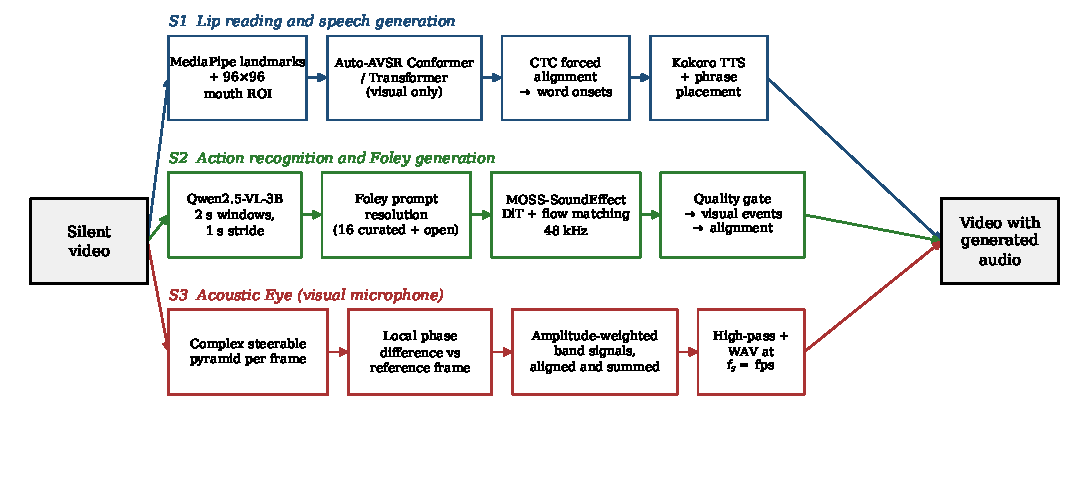
\includegraphics[width=\textwidth]{fig_arch.pdf}
\caption{System architecture. Three independent paths convert silent video to
audio. All three decode the video stream only; audio present in the source
container is never read. Each model runs in its own virtual environment as a
subprocess, so no two models are ever resident in the same interpreter or at the
same time.}
\label{fig:arch}
\end{figure*}

\subsection{Process isolation}

Fig.~\ref{fig:arch} shows the overall structure. The three paths impose mutually
incompatible requirements: S1 needs Python 3.11 with torchvision 0.20.1 (whose
video reader was removed in later releases) and \texttt{numpy<2} for MediaPipe
\cite{mediapipe2019}, while S2 needs Python 3.12 with torch 2.9.1, and its
text-to-speech component needs \texttt{numpy>=2}. These cannot coexist in one
interpreter.

Models are therefore invoked as subprocesses in separate virtual environments,
never imported into the long-lived API process. Three consequences follow, all
deliberate. Memory is released unconditionally at process exit, which is more
reliable than garbage collection combined with \texttt{torch.mps.empty\_cache()};
this matters because Qwen2.5-VL peaks near 12\,GB and MOSS near 12.1\,GB on a
17\,GB machine. Dependencies are isolated. And a model crash returns a non-zero
exit code that is converted to a readable message rather than taking down the
server.

\subsection{The nine-stage pipeline (S2)}

The S2 path runs as nine stages: upload, validation, action recognition, timeline
resolution, Foley generation, Foley quality validation, visual synchronisation,
audio mixing, and rendering. Each stage reports real state to a job store that is
persisted to disk after every transition. Progress within action recognition is
derived from a file the runner writes per window, so the reported percentage
tracks completed work rather than elapsed time.

Validation rejects files with no video stream, duration outside
$[0.4, 60]$\,s, size above 200\,MB, or a disallowed extension. A video that
already carries an audio track is accepted with a warning; the stream is never
decoded.

\subsection{Action timeline}

Qwen2.5-VL is run over 2.0\,s windows at 1.0\,s stride, eight frames per window
resized to $448\times252$, in bfloat16 on MPS. Each window is described
independently and the response is parsed into an action phrase and its verb head.
Windows sharing a head are merged into spans.

Because the stride is half the window, raw spans overlap by one stride: for the
reference clip, \emph{pick up cup} spans 2.0--6.0\,s and \emph{drink from cup}
spans 5.0--9.0\,s, sharing a second. An instant belonging to two actions is
ambiguous for audio placement, so spans are resolved to a non-overlapping timeline
by midpoint boundary resolution. Segments supported by few windows are flagged
\texttt{suspect} rather than deleted, and surface in the interface as medium
confidence.

\subsection{Foley class resolution}

A resolved action phrase is mapped to a Foley specification comprising a
generation prompt, a negative prompt, a synchronisation strategy, a frame region
in which to measure motion, an asset selection rule, and a target level.
Resolution proceeds in tiers: 16 hand-tuned curated classes are matched first,
then a set of deliberately silent actions (standing, reaching, holding), then a
verb-plus-object fallback to generic placement, pickup or press classes.

The ordering is load-bearing. An earlier version matched on bare keywords such as
\texttt{place} and \texttt{pick}, which caused ``place spoon on table'' to inherit
ceramic-mug Foley. Every curated keyword now names its object, and generic classes
are tried only after specific ones. That precision opened a different hole:
``place bread in toaster'' is unmistakably a placement but contains none of the
literal surfaces the generic keywords required, so it resolved to nothing and the
job failed before reaching the audio model. The verb fallback closes that hole
while running last, so specific classes and deliberate silences still win.

A final open-vocabulary tier synthesises a specification for any phrase not
otherwise matched. It classifies the phrase's verb into one of nine archetypes
(locomotion, impact, placement, pickup, mechanism, friction, liquid, oral,
ambient), each of which determines the synchronisation strategy, region, selection
rule and level, and composes a prompt from the archetype's acoustic description
and the literal action phrase. An unrecognised verb defaults to a continuous
ambient texture rather than a sharp transient, because a misplaced texture is far
less jarring than a misplaced impact. Synthesis is deterministic, so the same
phrase always produces the same prompt and the content-addressed cache remains
meaningful; keys are formed from archetype and object, so ``kick the ball'' and
``kicking a football'' share one generation.

\subsection{Foley generation}
\label{sec:phases}

Generation runs in three memory-separated phases so the components are never
co-resident: the Qwen3 text encoder (3.44\,GB), the Diffusion Transformer
(2.85\,GB), and the DAC decoder (0.74\,GB). Parameters are cast to bfloat16 but
buffers are left untouched, because the Transformer carries complex rotary
position tables that a blanket cast would destroy. One embedding function is
redirected to CPU because it computes in float64, which MPS does not support.
Both adaptations live in a wrapper; the upstream repository is unmodified, which
is verified by requiring \texttt{git status --porcelain} to return empty.

Assets are cached by a SHA-256 over the action key, both prompts, seed, step
count, guidance scale, sigma shift, duration and sample rate, truncated to 16 hex
characters. Numeric values are normalised before hashing --- without this, a
client sending \texttt{duration: 10} and a default of \texttt{10.0} produce
different keys for byte-identical audio.

%=====================================================================
\section{Foley Quality Validation}
\label{sec:gate}
%=====================================================================

Every generated asset is measured in its raw state, before any gain or
normalisation, and must clear six gates to enter the mix:

\begin{enumerate}
\item effective bits $\geq 9.0$, where effective bits is
      $16 + \log_2(\mathrm{peak})$, rejecting material whose peak is below
      about $-42$\,dBFS;
\item dynamic range $\geq 6$\,dB, measured over signal-bearing frames only;
\item not a sustained tone: harmonic ratio $> 0.80$ combined with dynamic
      range $< 10$\,dB;
\item not a pure tone: harmonic ratio $> 0.90$ combined with spectral
      flatness $< 0.01$;
\item required make-up gain $\leq +25$\,dB;
\item integrity: finite samples, correct sample rate, duration $\geq 0.05$\,s.
\end{enumerate}

Two of these thresholds were set by specific observed failures. Gate~4 exists
because gate~3 alone missed the 346\,Hz sine described in
Section~\ref{sec:existing}: that file had 32\,dB of dynamic range, so the
combined tonality test did not fire. A tone with a natural envelope is still a
tone, and inharmonicity is disqualifying on its own.

The dynamic-range measurement in gate~2 requires care. Computing it over all
frames including exact digital silence sends the fifth percentile to the numeric
floor and returns values of 183--201\,dB, which is physically impossible for
16-bit audio and scores full marks. A file that is 90\,\% silence with a few
clicks would pass as excellent. The measurement is therefore restricted to frames
above $-70$\,dB relative to the frame maximum, and capped at 96\,dB.

Passing candidates are ranked by a score in $[0,100]$ combining dynamic range (40
points), signal level (25), gain headroom (20) and non-tonality (15). Up to three
candidates are generated with successive seeds, stopping early once one scores at
least 45, so a class that works on the first seed costs exactly one generation.

A rejected asset never reaches the mixer. Its interval is marked
\texttt{no\_usable\_foley} and left silent, the measured values and reason are
recorded in the job result, the file is kept on disk for diagnostics, and
processing continues for every other action. If every asset is rejected the video
is still produced, with a silent track. The mixer holds an independent second
limit: no clip is amplified by more than $+25$\,dB, and a clip needing more is
refused rather than clamped, because clamping still admits amplified noise.

%=====================================================================
\section{Visual Event Localisation and Alignment}
%=====================================================================

This is the stage that makes the output correct rather than merely present.

Frames are decoded to $320\times180$ greyscale at 24\,fps and motion is computed
as the mean absolute inter-frame difference within a horizontal band of the
frame. Four bands are defined as fractions of frame height: feet (0.62--1.00),
head (0.00--0.50), table (0.40--0.85) and full (0.00--1.00). Let $I_t$ denote
frame $t$ restricted to band $b$; the motion signal is

\begin{equation}
m_b(t) = \frac{1}{|B|}\sum_{p \in B} \left| I_t(p) - I_{t-1}(p) \right|
\label{eq:motion}
\end{equation}

smoothed before peak analysis. The band restriction in \eqref{eq:motion} is what
makes the signal usable: measuring motion over the whole frame mixes a footstep
into arm and head movement, whereas the feet band responds almost exclusively to
gait.

The detection rule depends on the physics of the action, not on the object:

\begin{itemize}
\item \textbf{footstep}: a prominence peak followed to its subsequent minimum.
      The swing of the leg is the peak; the \emph{plant} is what is audible.
\item \textbf{hold}: a sustained motion minimum. A sip is the vessel held still
      at the lips, so it is a minimum rather than a peak.
\item \textbf{contact}: the final motion peak before rest, where the object meets
      the surface as movement stops.
\item \textbf{continuous}: the whole interval, where no discrete instant exists.
\end{itemize}

Fig.~\ref{fig:motion} shows the three relevant bands for the reference clip with
the detected events overlaid.

\begin{figure*}[t]
\centering
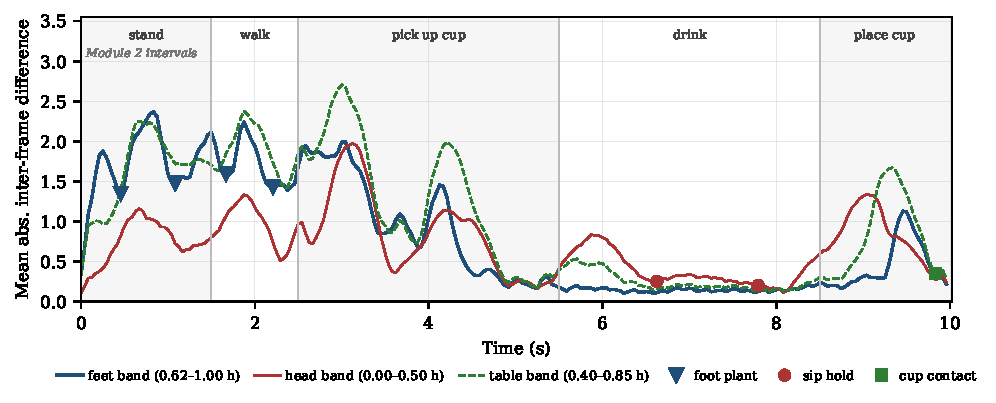
\includegraphics[width=\textwidth]{fig_motion.pdf}
\caption{Region-band motion signals for the reference clip, with the visual
events derived from them. Feet-band motion during the interval Module~2 labels
\emph{stand} (mean 1.708) is statistically indistinguishable from the labelled
\emph{walk} interval (1.711), and two of the four foot plants fall inside the
\emph{stand} label. Drinking is by a wide margin the least visually active
interval, which is why sip holds are detected as motion minima rather than peaks.}
\label{fig:motion}
\end{figure*}

\subsection{Alignment uses true attack times}

Once a visual instant is known, the generated clip must be positioned so that its
audible transient coincides with it. An early implementation aligned
onset-\emph{strength} peaks, which is incorrect: an onset-strength peak marks
where spectral flux is greatest, not where the transient begins, and it leads or
lags the true attack by $-96$ to $+250$\,ms. One asset footstep reported at
3.760\,s in fact attacks at 3.856\,s, so aligning the strength peak misplaced the
audible sound by exactly 96\,ms --- an error that was audible in the rendered
output before it was found.

Alignment therefore uses the true envelope attack: the amplitude envelope
maximum, back-tracked to the last point at which it rose through 20\,\% of that
maximum. Clips are shifted, never time-stretched. Where the generated cadence
differs from the filmed one the residual is absorbed and reported, because
correcting it would alter the character of the audio.

\subsection{Mixing}

Per clip, in order: DC removal, cut points snapped to the nearest zero crossing
within $\pm3$\,ms, 12\,ms raised-cosine fades, level set by active RMS against the
class target, and a peak cap at $-6$\,dBFS. Levels differ by class by design: a
mug meeting a table is percussive, footsteps are mid-ground, and a sip is
intimate, so normalising all three to equal loudness would not correspond to any
real recording position. The peak cap is an outlier guard, not a leveller; at
$-12$\,dBFS it bound on most clips and flattened the dynamics between events,
which is why it was raised.

The bus sums, normalises linearly to $-6$\,dBFS, and passes through a safety
limiter (threshold $-6$, ceiling $-3$) whose gain reduction is always reported.

%=====================================================================
\section{Experimental Setup}
%=====================================================================

All experiments ran on one machine: Apple M4, 17.18\,GB unified memory,
macOS~26.2, PyTorch~2.9.1 with MPS. There is no CUDA path. Software versions are
pinned per environment as described in Section~\ref{sec:existing}.

The reference clip for S2 is a 10.005\,s, $1280\times720$, 24\,fps recording of a
person walking to a table, picking up a cup, drinking twice and placing the cup
down. It is held under a recorded SHA-256 and was not modified during
development. S1 was evaluated on seven recordings of 59--98 frames.

Measurements come from four sources, none of which involved regenerating audio
for the purpose of this paper:

\begin{itemize}
\item \textbf{Job records.} 32 completed pipeline runs persisted to disk, each
      containing per-event alignment residuals recorded at render time.
\item \textbf{Generation records.} 38 generation runs, of which 31 used
      production settings, each recording per-phase timing and memory.
\item \textbf{The asset corpus.} All 54 audio files produced during development,
      re-measured with the production validator.
\item \textbf{Test suites.} 64 automated tests, executed for this paper.
\end{itemize}

The synthetic vibration experiment for S3 was run specifically for this paper and
is described in Section~\ref{sec:vmresults}.

%=====================================================================
\section{Results and Discussion}
\label{sec:results}
%=====================================================================

\subsection{Functional verification}

Both automated suites pass in full: 42 tests covering configuration, prompt
resolution, video validation, the job state machine, synchronisation, mixing,
rendering and the API surface; and 22 tests covering the quality gate and
candidate selection. An end-to-end gate over the reference clip completes with
five actions detected, four Foley classes generated, zero assets rejected, five
placements written to the mix, and one interval (\emph{stand}) deliberately
silent. The gate additionally asserts that no rejected asset reached the mix.

The generalised synchronisation service reproduces the validated reference
implementation exactly --- foot plants at $[0.458, 1.083, 1.667, 2.208]$\,s, sip
holds at $[6.625, 7.792]$\,s and cup contact at $9.833$\,s --- and this is
asserted in the test suite rather than checked by hand. The band statistics
recomputed for Fig.~\ref{fig:motion} reproduce the recorded values to three
decimal places.

\subsection{Synchronisation accuracy}

Table~\ref{tab:sync} reports the synchronisation errors for the validated build,
measured on the \emph{rendered audio} by detecting envelope attacks in the final
WAV and comparing against the visual event timestamps. This is a stronger
measurement than reading the alignment plan, because it includes any error
introduced by segment selection, fades and mixing.

\begin{table}[t]
\caption{Synchronisation error measured on the rendered audio of the validated
build. One frame at 24\,fps is 41.7\,ms.}
\label{tab:sync}
\centering
\small
\begin{tabular}{@{}llcc@{}}
\toprule
\textbf{Action} & \textbf{Visual event} & \textbf{Rendered attack} & \textbf{Error} \\
\midrule
Walk (plant 1) & 0.458\,s & 0.458\,s & $-0$\,ms \\
Walk (plant 2) & 1.083\,s & 1.063\,s & $-20$\,ms \\
Walk (plant 3) & 1.667\,s & 1.675\,s & $+8$\,ms \\
Walk (plant 4) & 2.208\,s & 2.221\,s & $+13$\,ms \\
Drink (hold 1) & 6.625\,s & 6.638\,s & $+13$\,ms \\
Drink (hold 2) & 7.792\,s & 7.803\,s & $+11$\,ms \\
Place cup      & 9.833\,s & 9.833\,s & $-0$\,ms \\
\bottomrule
\end{tabular}
\end{table}

The worst error is 20\,ms, below the 20.8\,ms half-frame interval at 24\,fps. All
seven events are within half a frame. We stress that this is one clip with seven
events, evaluated on the build that was tuned on it; it demonstrates that the
method can achieve sub-frame placement, not that it does so in general.

\subsection{Why alignment error accumulates}
\label{sec:cadence}

The alignment residuals recorded across job runs are deterministic per asset,
which permits a more informative analysis than an aggregate. Fig.~\ref{fig:cadence}
shows the cause.

\begin{figure*}[t]
\centering
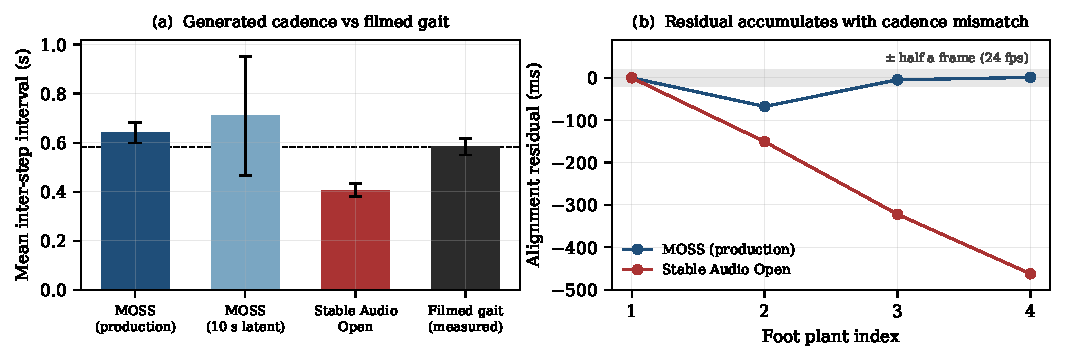
\includegraphics[width=\textwidth]{fig_cadence.pdf}
\caption{(a) Mean inter-step interval of each walking asset compared with the
filmed gait, with standard deviation. (b) Per-plant alignment residual for the
two production backends. Because clips are shifted and never stretched, a
mismatch between generated cadence and filmed cadence accumulates across
successive contacts.}
\label{fig:cadence}
\end{figure*}

The filmed gait has a mean inter-step interval of 0.583\,s
($\sigma = 0.034$\,s). The MOSS walking asset generates steps at 0.641\,s
($\sigma = 0.042$\,s), 9.9\,\% slower, and its residuals stay within
$[0, -67.6]$\,ms across four plants. The Stable Audio asset generates at 0.407\,s
($\sigma = 0.026$\,s), 30.2\,\% faster, and its residual grows monotonically to
$-462.4$\,ms by the fourth plant. That growth is predictable from the assets
alone: three step intervals at a 0.176\,s deficit accumulate to 0.528\,s, and
0.462\,s was observed after the matcher selected the best-fitting run.

This is a direct consequence of the shift-only policy and is the clearest
argument for its limits. Shifting preserves the character of the generated audio
but cannot correct a cadence mismatch, so alignment quality for rhythmic actions
depends on the generator producing a plausible tempo. It also gives an objective,
timing-based reason to prefer MOSS for this material that is independent of the
harmonic-ratio argument in Section~\ref{sec:existing}.

\subsection{Quality gate ablation}
\label{sec:gateresults}

All 54 assets produced during development were re-measured with the production
validator. The gate rejects 16 of them, 29.6\,\% of the corpus.
Fig.~\ref{fig:gate} shows the corpus in the plane of the two most discriminating
metrics.

\begin{figure}[t]
\centering
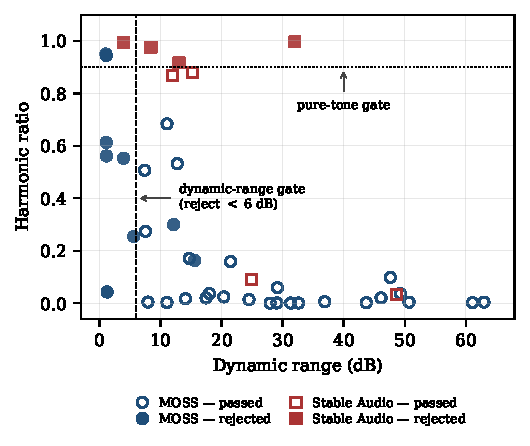
\includegraphics[width=\columnwidth]{fig_gate.pdf}
\caption{All 54 generated assets in the dynamic-range / harmonic-ratio plane.
Filled markers were rejected. The Stable Audio cluster at harmonic ratio near 1.0
consists of near-pure tones; the two at 32\,dB and 12\,dB of dynamic range would
have passed a dynamic-range test alone.}
\label{fig:gate}
\end{figure}

Had the gate not existed, all 16 would have reached the mixer. Eleven of them
would have required more than the $+25$\,dB mixer limit, with a median required
gain of $+29.1$\,dB and a maximum of $+42.1$\,dB. Applying $+42$\,dB to a file
whose peak is $-62$\,dBFS does not produce a quiet contact sound; it produces
amplified quantisation noise.

The backend split is informative. Of 46 MOSS assets, 12 were rejected (26\,\%);
of 8 Stable Audio assets, 4 were rejected (50\,\%). Median quality scores are
almost identical --- 54.5 for MOSS against 53.2 for Stable Audio --- while median
harmonic ratio differs by a factor of 22, at 0.040 against 0.898. The aggregate
score does not separate these backends; the harmonic ratio separates them
decisively. This is the empirical case for multi-criteria gating: a single scalar,
however carefully weighted, can be blind to the failure that matters.

Ten assets have a harmonic ratio above 0.80. The two most extreme, both Stable
Audio cup placements, measure 0.997 and 0.995 with spectral flatness of $0.00000$
--- pure sine waves. Two assets at 0.880 and 0.868 pass, which indicates the gate
has a real boundary rather than rejecting everything tonal.

\subsection{Generation settings: what the metrics miss}

Two speed-ups were tried during development and reverted after listening.
Table~\ref{tab:ablation} quantifies both.

\begin{table}[t]
\caption{Generation-settings ablation. The aggregate score is insensitive to the
step reduction and moves in a misleading direction for the latent reduction,
while the structural measure detects the degradation.}
\label{tab:ablation}
\centering
\small
\begin{tabular}{@{}lrrrrr@{}}
\toprule
\textbf{Setting} & \textbf{Gen (s)} & \textbf{Score} & \textbf{Dyn (dB)} & \textbf{Attacks} & \textbf{Gap $\sigma$} \\
\midrule
\multicolumn{6}{@{}l}{\textit{(a) Denoising steps --- impact class}}\\
50 steps (prod.) & 266 & 86.9 & 32.6 & 7 & --- \\
35 steps         & 200 & 86.3 & 31.3 & 7 & --- \\
25 steps         & 129 & 86.4 & 29.1 & 7 & --- \\
\midrule
\multicolumn{6}{@{}l}{\textit{(b) Denoised latent length --- walking class}}\\
30\,s (prod.) & 242 & 97.1 & 43.7 & 16 & 0.042 \\
10\,s         &  88 & 86.0 & 61.1 &  8 & 0.244 \\
\midrule
Filmed gait   & --- & --- & --- & 4 & 0.034 \\
\bottomrule
\end{tabular}
\end{table}

Reducing the step count from 50 to 25 halves generation time and moves the
quality score by 0.6 points, within noise. The transient count is unchanged. The
gate is effectively blind to this change, and the decision to revert it rests
entirely on listening.

The latent reduction is more revealing. Cutting the denoised window from 30\,s to
10\,s makes generation 2.8$\times$ faster and \emph{raises} both the measured
dynamic range (43.7 to 61.1\,dB) and the effective bits (14.9 to 16.0) --- both
of which the score rewards. Yet the number of detectable transients falls from 16
to 8, and the standard deviation of inter-step intervals rises from 0.042\,s to
0.244\,s, a factor of 5.8. Fig.~\ref{fig:latent} shows the two envelopes. The
production asset is a regular gait; the ablated asset is a sparse, irregular
sequence. It also explains the single-plant alignment observed in the one job run
that used the shortened latent: with only eight irregular transients, the matcher
could not find a run of four that fitted the filmed gait.

\begin{figure}[t]
\centering
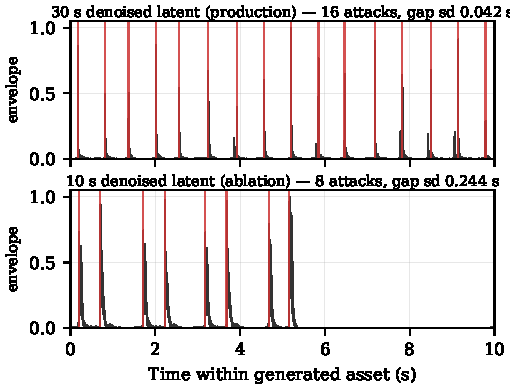
\includegraphics[width=\columnwidth]{fig_latent.pdf}
\caption{Amplitude envelope of the walking asset generated with the production
30\,s latent (top) and the 10\,s ablation (bottom). Vertical lines mark detected
attacks. The ablated asset has half as many transients and 5.8$\times$ the
inter-step irregularity, while scoring higher on dynamic range.}
\label{fig:latent}
\end{figure}

The effect on the hardest class is decisive. Cup pickup is the class for which
multi-candidate generation exists. With the 30\,s latent, one of three seeds
passes the gate (seed 44, score 86.6). With the 10\,s latent, \emph{none} of the
three passes; peaks sit at $-33$\,dBFS and all three would need over $+40$\,dB of
gain. The speed-up would have made the hardest class permanently silent.

The general lesson is that an aggregate score computed from marginal statistics
can improve while the temporal structure that makes audio usable is destroyed. A
structural measure --- how many transients are present and how regularly they are
spaced --- captures what the scalar misses, and is cheap to compute.

\subsection{Acoustic Eye: controlled characterisation}
\label{sec:vmresults}

The vibration path had no positive result on real footage, because the available
recordings are at 30--60\,fps and the recoverable band is bounded by half the
frame rate. To establish whether the implementation is correct, a synthetic
stimulus with known ground truth was constructed: a band-limited noise texture
translated sinusoidally by a known sub-pixel amplitude at a known frequency,
rendered at several frame rates. This is an optical test, not an acoustic capture.

\begin{figure*}[t]
\centering
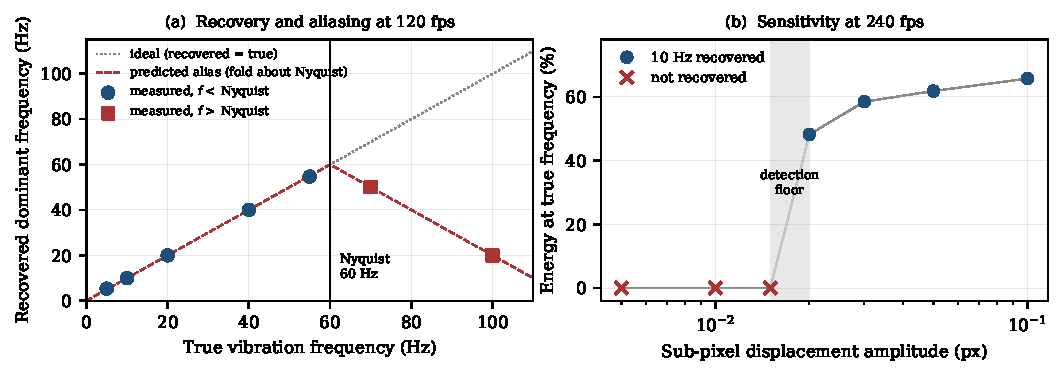
\includegraphics[width=\textwidth]{fig_vm.pdf}
\caption{Controlled characterisation of the visual microphone on synthetic
stimuli. (a) At 120\,fps, frequencies below Nyquist are recovered exactly, and
frequencies above it fold about Nyquist exactly as the dashed prediction
requires. (b) Recovery at 240\,fps degrades sharply between 0.020\,px and
0.015\,px of displacement.}
\label{fig:vm}
\end{figure*}

The results, shown in Fig.~\ref{fig:vm}, are unambiguous. A 10\,Hz oscillation of
0.30\,px amplitude is recovered with zero frequency error at every frame rate
from 30 to 480\,fps, carrying 65--66\,\% of the spectral energy above 0.5\,Hz. At
120\,fps, signals at 5, 10, 20, 40 and 55\,Hz are recovered exactly; signals at 70
and 100\,Hz fold to 50 and 20\,Hz respectively, matching the aliasing prediction
to within measurement resolution. Sensitivity degrades sharply below 0.02\,px:
recovery is exact at 0.020\,px with 48.2\,\% of the energy at the true frequency,
and fails completely at 0.015\,px.

The implementation is therefore correct, and its limit on ordinary footage is the
sampling theorem rather than a defect. At 60\,fps the recoverable band ends at
30\,Hz, which excludes speech and essentially all musical content. The
recorded 60\,fps job produced a signal whose dominant component is at 0.06\,Hz,
which is camera drift, not sound. Reporting the system as a demonstrator of the
principle, subject to a stated frame-rate requirement, is the only honest
description.

Throughput was measured on the same machine: 1284 frames/s at $64\times64$,
441 frames/s at $128\times128$, and 103 frames/s at $256\times256$. Cost scales
with pixel count, as one steerable pyramid is constructed per frame.

\subsection{Latency and resource use}

Table~\ref{tab:latency} compiles timing from the recorded runs.

\begin{table}[t]
\caption{Measured latency and memory. S1 and S2 figures are means over 7 and 31
recorded runs respectively; S3 is measured on synthetic input.}
\label{tab:latency}
\centering
\small
\begin{tabular}{@{}llr@{}}
\toprule
\textbf{Path} & \textbf{Quantity} & \textbf{Measured} \\
\midrule
S1 & Model load & 0.5--0.7\,s \\
S1 & Inference (87 frames mean) & 1.57\,s \\
S1 & Total per clip & 3.73\,s \\
S1 & Real-time factor & 0.45$\times$ \\
\midrule
S2 & Phase 1 --- text encoder & 4.7\,s \\
S2 & Phase 2 --- diffusion (50 steps) & 264.4\,s \\
S2 & Phase 3 --- decode & 8.6\,s \\
S2 & Total per generated asset & 280.9\,s \\
S2 & Peak resident memory & 12.11\,GB \\
S2 & Minimum available memory & 2.35\,GB (worst 1.58) \\
S2 & Whole job, fully cached & 39.5\,s (median) \\
S2 & Whole job, with generation & 556.9\,s (median) \\
\midrule
S3 & Throughput, $128\times128$ & 441 frames/s \\
\bottomrule
\end{tabular}
\end{table}

S1 runs faster than real time on CPU. S2 is dominated by diffusion, which
consumes 94\,\% of generation time; because the model denoises a fixed-length
latent, a short request costs the same as a long one. Caching matters
accordingly: a fully cached job completes in about 40\,s against roughly nine
minutes when generation is required.

The memory figures deserve attention. Peak resident memory averaged 12.11\,GB
against a 17.18\,GB machine, and in the worst recorded run the available memory
fell to 1.58\,GB against a guard threshold of 1.50\,GB --- a margin of 80\,MB.
The memory guard was never breached across 31 recorded generations, and swap
growth was 0.00--0.01\,GB. The phase separation described in
Section~\ref{sec:phases} is what makes this fit; without it the three components
would be co-resident and the run would fail.

\subsection{Audio independence of the lip-reading path}

A claim that a system reads lips must be demonstrated rather than asserted. The
audio stream was stripped from a test recording with
\texttt{ffmpeg -map 0:v:0 -c:v copy -an} and the clip re-run. Decoded video
frames were bit-identical to the original, with a maximum pixel difference of 0
across $2.21 \times 10^{9}$ values; the model input tensor was bitwise identical;
and the output matched exactly, with the same sentence, token identifiers and
decoder score. The result is structural as well as empirical: the model frontend
is a 3-D convolutional stack accepting only $(B, T, 1, 88, 88)$ pixel tensors,
and cannot ingest a waveform.

\subsection{Input format sensitivity in S1}

Decoder confidence tracks input format closely, as shown in
Table~\ref{tab:format}. Auto-AVSR is trained on 25\,fps SDR video, and HDR
footage decoded without tone mapping shifts the pixel distribution far from the
training regime.

\begin{table}[t]
\caption{S1 decoder score against input format. Higher (less negative) is more
confident.}
\label{tab:format}
\centering
\small
\begin{tabular}{@{}lcc@{}}
\toprule
\textbf{Format} & \textbf{Input tensor mean} & \textbf{Best score} \\
\midrule
25\,fps SDR & 0.06 & $-0.36$ \\
30\,fps SDR & 0.57--0.61 & $-1.05$ \\
30\,fps HDR (HLG) & 1.24--1.29 & $-4.31$ \\
\bottomrule
\end{tabular}
\end{table}

The system standardises every upload to 25\,fps SDR and rejects HDR rather than
converting it, because a correct HLG-to-SDR conversion requires an FFmpeg filter
that is absent from many builds, and silently degrading accuracy is worse than
refusing the input. We note that these are decoder scores, not accuracy: they
indicate the model's confidence, and a confident wrong answer is possible.

%=====================================================================
\section{Limitations}
%=====================================================================

\textbf{Action recognition is the binding constraint on S2.} Foley can only be as
good as the timeline it is given. On a coffee-stirring test video, the recogniser
missed a cup placement entirely, emitted one stirring action under three
different labels, and returned a caption (``Stirring a cup of coffee'') rather
than an action. Fig.~\ref{fig:motion} shows a second instance: the interval
labelled \emph{stand} has feet-band motion of 1.708 against 1.711 in the labelled
\emph{walk}, and contains two of the four foot plants. The pipeline compensates by
widening the footstep search span, but the label itself is wrong.

\textbf{Synchronisation is validated on limited footage.} The 20\,ms result is
seven events on one clip, on the build tuned against it. Across the 32 recorded
job runs, only footstep placements record per-event residuals; hold and contact
placements record the aligned instant but not a residual, so the multi-clip
evidence is thinner than the number of runs suggests.

\textbf{No word error rate is reported for S1.} Ground-truth transcripts for the
test recordings were not retained, so recognition quality is characterised only
by decoder scores and by two spot-checked correct transcriptions. The published
checkpoint reports 20.3\,\% WER on LRS3; no claim is made that this system
reproduces that figure on its own material.

\textbf{Listening evaluation is single-assessor.} Every judgement that audio
``sounds right'' was made by the developer. No formal listening test with
multiple participants, randomised presentation or statistical analysis was
conducted. Given that Section~\ref{sec:gateresults} demonstrates objective
metrics failing to capture perceptible degradation, this is a substantive
limitation rather than a formality.

\textbf{S3 has not recovered real sound.} The characterisation in
Section~\ref{sec:vmresults} is synthetic. No real acoustic signal has been
recovered from real footage, because no high-speed camera was available.

\textbf{Output is sparse by nature.} For discrete object interactions,
roughly 18\,\% of a 10\,s timeline carries audio. The silence between events is
correct, but it means the result is not a continuous soundtrack.

\textbf{Apple Silicon only, single machine, single job.} The pipeline depends on
MPS with no CUDA or CPU fallback. Jobs run in process with no queue,
authentication or multi-user isolation. Video length is capped at 60\,s because
recognition cost grows linearly.

\textbf{Comparative evaluation is limited.} No comparison against Diff-Foley,
MMAudio or FoleyCrafter on a standard benchmark with standard metrics was
performed. The rejections in Section~\ref{sec:existing} are measurements on this
project's own material and hardware, and should not be read as general statements
about those systems.

%=====================================================================
\section{Future Work}
%=====================================================================

The most valuable next step is improving the action timeline, since it bounds
everything downstream in S2. Two directions are concrete: prompt engineering for
the vision-language model to elicit action phrases rather than captions, and
label normalisation to merge synonymous predictions across windows.

A second direction is a formal listening evaluation with multiple assessors,
randomised presentation and a pairwise design. The finding that scores are
insensitive to audible degradation makes a perceptual study the only way to
validate the quality gate's thresholds.

Third, the shift-only alignment policy could be relaxed for rhythmic actions.
Section~\ref{sec:cadence} shows that residual accumulation is driven by cadence
mismatch; selecting among several generated candidates by cadence fit, rather than
by quality score alone, would address this without time-stretching.

Fourth, the visual microphone path should be evaluated on genuine high-speed
footage. The synthetic characterisation establishes the implementation is
correct; a 240\,fps capture of a loud source next to a light, resonant object is
the natural test.

Finally, a comparison against Diff-Foley, MMAudio and FoleyCrafter on VGGSound or
a comparable benchmark, reporting Fréchet Audio Distance alongside onset accuracy,
would place the alignment method in context.

%=====================================================================
\section{Conclusion}
%=====================================================================

This paper described a system that reconstructs audio from silent video along
three paths --- visual speech recognition with timed synthesis, action
recognition with aligned Foley generation, and phase-based vibration recovery ---
running entirely on a single consumer laptop.

The central finding is that in generated-Foley systems, placement and validation
matter as much as generation. Anchoring generated audio to visually measured
contact instants using true envelope attack times achieved a worst-case error of
20\,ms on the reference clip, within half a frame at 24\,fps. Measuring every
generated asset before mixing rejected 29.6\,\% of the development corpus, eleven
items of which would otherwise have received more than $+25$\,dB of automatic
gain.

Two results argue against trusting aggregate audio quality scores. Two backends
with nearly identical median scores, 54.5 and 53.2, differ in median harmonic
ratio by a factor of 22, one of them producing pure sine waves for object
contacts. And a generation setting that raised measured dynamic range from 43.7 to
61.1\,dB simultaneously halved the number of detectable transients and made a
class that previously produced one usable candidate in three produce none. In
both cases a structural measure caught what the scalar missed.

The system is a demonstrator with real limits, and they have been stated: action
recognition is the weakest component, synchronisation is validated on limited
footage, the listening evaluation has one assessor, and the vibration path has
been characterised only on synthetic stimuli. Within those limits, the work shows
that a laptop-scale pipeline can place generated sound accurately enough to
survive frame-level scrutiny, provided the audio it generates is measured before
it is believed.

%=====================================================================
\begin{thebibliography}{00}

\bibitem{owens2016}
A.~Owens, P.~Isola, J.~McDermott, A.~Torralba, E.~H. Adelson, and W.~T. Freeman,
``Visually indicated sounds,'' in \emph{Proc. IEEE Conf. Comput. Vis. Pattern
Recognit. (CVPR)}, 2016, pp. 2405--2413.

\bibitem{diffoley2023}
S.~Luo, C.~Yan, C.~Hu, and H.~Zhao, ``Diff-Foley: Synchronized video-to-audio
synthesis with latent diffusion models,'' in \emph{Adv. Neural Inf. Process.
Syst. (NeurIPS)}, vol.~36, 2023.

\bibitem{foleycrafter2024}
Y.~Zhang, Y.~Gu, Y.~Zeng, Z.~Xing, Y.~Wang, Z.~Wu, and K.~Chen, ``FoleyCrafter:
Bring silent videos to life with lifelike and synchronized sounds,''
\emph{arXiv:2407.01494}, 2024.

\bibitem{mmaudio2025}
H.~K. Cheng, M.~Ishii, A.~Hayakawa, T.~Shibuya, A.~Schwing, and Y.~Mitsufuji,
``MMAudio: Taming multimodal joint training for high-quality video-to-audio
synthesis,'' in \emph{Proc. IEEE/CVF Conf. Comput. Vis. Pattern Recognit.
(CVPR)}, 2025, pp. 28901--28911.

\bibitem{audioldm2}
H.~Liu, Y.~Yuan, X.~Liu, X.~Mei, Q.~Kong, Q.~Tian, Y.~Wang, W.~Wang, Y.~Wang,
and M.~D. Plumbley, ``AudioLDM 2: Learning holistic audio generation with
self-supervised pretraining,'' \emph{IEEE/ACM Trans. Audio, Speech, Language
Process.}, vol.~32, pp. 2871--2883, 2024.

\bibitem{stableaudio2024}
Z.~Evans, J.~D. Parker, C.~Carr, Z.~Zukowski, J.~Taylor, and J.~Pons, ``Stable
Audio Open,'' \emph{arXiv:2407.14358}, 2024.

\bibitem{moss2026}
OpenMOSS Team, ``MOSS-SoundEffect v2.0,'' 2026. [Online]. Available:
\url{https://huggingface.co/OpenMOSS-Team/MOSS-SoundEffect-v2.0}

\bibitem{dac2023}
R.~Kumar, P.~Seetharaman, A.~Luebs, I.~Kumar, and K.~Kumar, ``High-fidelity audio
compression with improved RVQGAN,'' in \emph{Adv. Neural Inf. Process. Syst.
(NeurIPS)}, vol.~36, 2023.

\bibitem{dit2023}
W.~Peebles and S.~Xie, ``Scalable diffusion models with transformers,'' in
\emph{Proc. IEEE/CVF Int. Conf. Comput. Vis. (ICCV)}, 2023, pp. 4195--4205.

\bibitem{flowmatching2023}
Y.~Lipman, R.~T.~Q. Chen, H.~Ben-Hamu, M.~Nickel, and M.~Le, ``Flow matching for
generative modeling,'' in \emph{Proc. Int. Conf. Learn. Represent. (ICLR)}, 2023.

\bibitem{afouras2018}
T.~Afouras, J.~S. Chung, A.~Senior, O.~Vinyals, and A.~Zisserman, ``Deep
audio-visual speech recognition,'' \emph{IEEE Trans. Pattern Anal. Mach.
Intell.}, 2018, doi: 10.1109/TPAMI.2018.2889052.

\bibitem{avhubert2022}
B.~Shi, W.-N. Hsu, K.~Lakhotia, and A.~Mohamed, ``Learning audio-visual speech
representation by masked multimodal cluster prediction,'' in \emph{Proc. Int.
Conf. Learn. Represent. (ICLR)}, 2022.

\bibitem{autoavsr2023}
P.~Ma, A.~Haliassos, A.~Fernandez-Lopez, H.~Chen, S.~Petridis, and M.~Pantic,
``Auto-AVSR: Audio-visual speech recognition with automatic labels,'' in
\emph{Proc. IEEE Int. Conf. Acoust., Speech, Signal Process. (ICASSP)}, 2023.

\bibitem{conformer2020}
A.~Gulati, J.~Qin, C.-C. Chiu, N.~Parmar, Y.~Zhang, J.~Yu, W.~Han, S.~Wang,
Z.~Zhang, Y.~Wu, and R.~Pang, ``Conformer: Convolution-augmented transformer for
speech recognition,'' in \emph{Proc. Interspeech}, 2020, pp. 5036--5040.

\bibitem{ctc2006}
A.~Graves, S.~Fern\'{a}ndez, F.~Gomez, and J.~Schmidhuber, ``Connectionist
temporal classification: Labelling unsegmented sequence data with recurrent
neural networks,'' in \emph{Proc. Int. Conf. Mach. Learn. (ICML)}, 2006, pp.
369--376.

\bibitem{visualmic2014}
A.~Davis, M.~Rubinstein, N.~Wadhwa, G.~J. Mysore, F.~Durand, and W.~T. Freeman,
``The visual microphone: Passive recovery of sound from video,'' \emph{ACM Trans.
Graph.}, vol.~33, no.~4, pp. 1--10, 2014.

\bibitem{phasebased2013}
N.~Wadhwa, M.~Rubinstein, F.~Durand, and W.~T. Freeman, ``Phase-based video
motion processing,'' \emph{ACM Trans. Graph.}, vol.~32, no.~4, pp. 1--10, 2013.

\bibitem{steerable1995}
E.~P. Simoncelli and W.~T. Freeman, ``The steerable pyramid: A flexible
architecture for multi-scale derivative computation,'' in \emph{Proc. IEEE Int.
Conf. Image Process. (ICIP)}, 1995, pp. 444--447.

\bibitem{fad2019}
K.~Kilgour, M.~Zuluaga, D.~Roblek, and M.~Sharifi, ``Fr\'{e}chet audio distance:
A reference-free metric for evaluating music enhancement algorithms,'' in
\emph{Proc. Interspeech}, 2019, pp. 2350--2354.

\bibitem{videomae2022}
Z.~Tong, Y.~Song, J.~Wang, and L.~Wang, ``VideoMAE: Masked autoencoders are
data-efficient learners for self-supervised video pre-training,'' in \emph{Adv.
Neural Inf. Process. Syst. (NeurIPS)}, vol.~35, 2022.

\bibitem{xclip2022}
B.~Ni, H.~Peng, M.~Chen, S.~Zhang, G.~Meng, J.~Fu, S.~Xiang, and H.~Ling,
``Expanding language-image pretrained models for general video recognition,'' in
\emph{Proc. Eur. Conf. Comput. Vis. (ECCV)}, 2022, pp. 1--18.

\bibitem{qwen25vl2025}
S.~Bai \emph{et al.}, ``Qwen2.5-VL technical report,''
\emph{arXiv:2502.13923}, 2025.

\bibitem{mediapipe2019}
C.~Lugaresi \emph{et al.}, ``MediaPipe: A framework for building perception
pipelines,'' \emph{arXiv:1906.08172}, 2019.

\end{thebibliography}

\end{document}
